\usetikzlibrary{automata,positioning,arrows}

\tikzset{
    ->, 
>=stealth, 
node distance=5cm,
every state/.style={thick, fill=gray!10},
initial text=$ $,}

\begin{figure}[H]
    \centering
    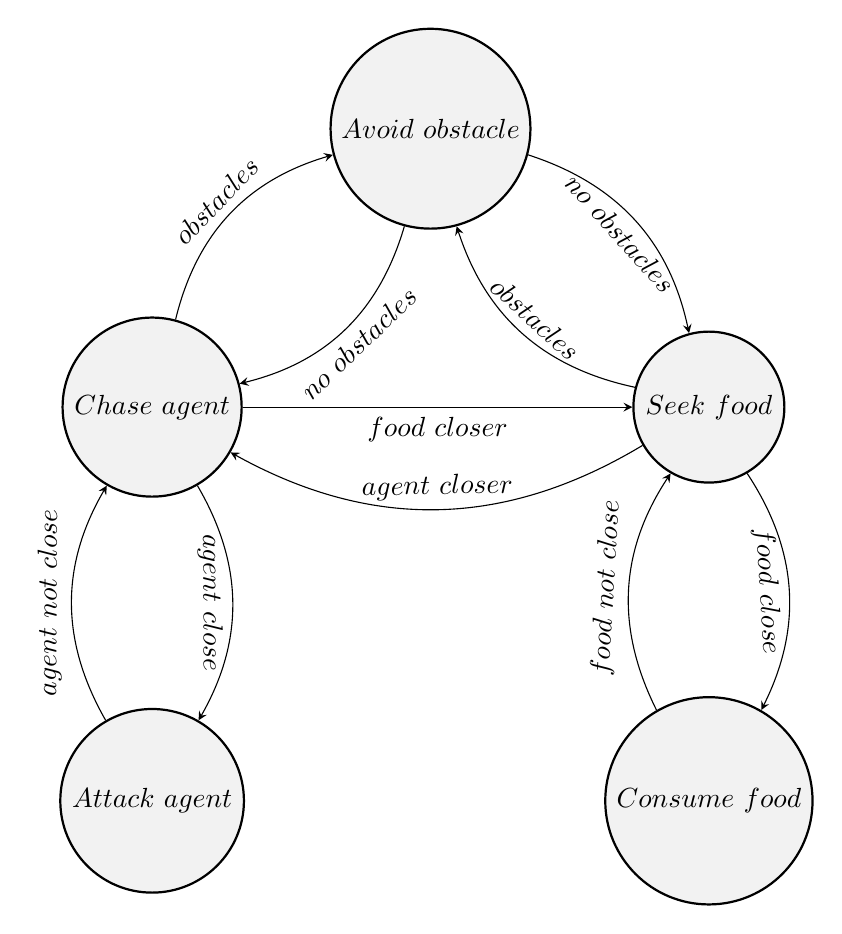
\begin{tikzpicture}
        \node[state] (1) {$Avoid\ obstacle$};
        \node[state, below left of=1] (2) {$Chase\ agent$};
        \node[state, below right of=1] (3) {$Seek\ food$};
        \node[state, below of=2] (4) {$Attack\ agent$};
        \node[state, below of=3] (5) {$Consume\ food$};
        \draw
        (1) edge[sloped, anchor=center, below, bend left] node{$no\ obstacles$} (3)
        (3) edge[sloped, anchor=center, above, bend left] node{$obstacles$} (1)
        (1) edge[sloped, anchor=center, below, bend left] node{$no\ obstacles$} (2)
        (2) edge[sloped, anchor=center, above, bend left] node{$obstacles$} (1)
        (2) edge[sloped, anchor=center, below, bend left] node{$agent\ close$} (4)
        (4) edge[sloped, anchor=center, above, bend left] node{$agent\ not\ close$} (2)
        (3) edge[sloped, anchor=center, below, bend left] node{$food\ close$} (5)
        (5) edge[sloped, anchor=center, above, bend left] node{$food\ not\ close$} (3)
        (2) edge[sloped, anchor=center, below] node{$food\ closer$} (3)
        (3) edge[sloped, anchor=center, above, bend left] node{$agent\ closer$} (2)
        ;
    \end{tikzpicture}
    \caption{Enemy FSM}
    \label{fig:enemy_FSM}
\end{figure}


